\chapter{Recurrent Neural Networks}\label{ch:rnn}

\section{Recurrent Neural Networks}
\begin{figure}
	\begin{center}
		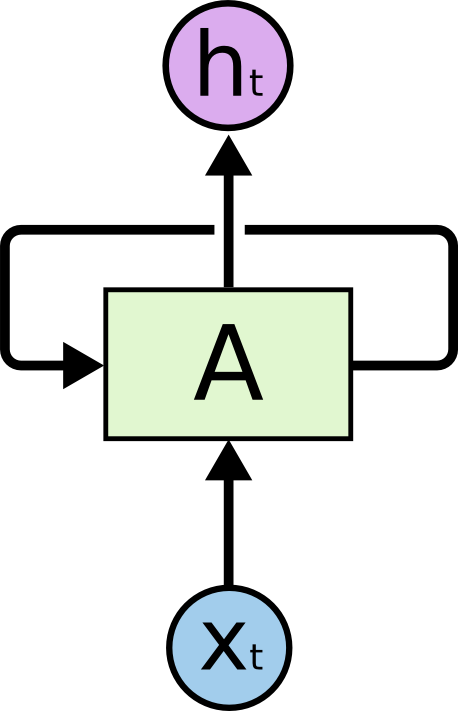
\includegraphics[scale=0.5]{rnn/rnn_rolled}
	\end{center}
	\caption{A recurrent neural network. From~\cite{olah2015understanding}\label{fig:rnn_img}}
\end{figure}

A recurrent neural network is a variation of an artificial neural network that continuously uses the output of its previous cell as the input of the current cell along with the input that was applied to this cell (see figure~\ref{fig:rnn_img}). Due to this feature, RNNs have the ability to store processed information from the previous input in the hidden state as these can be passed along through the previous cell's output. 

\begin{figure}
	\begin{center}
		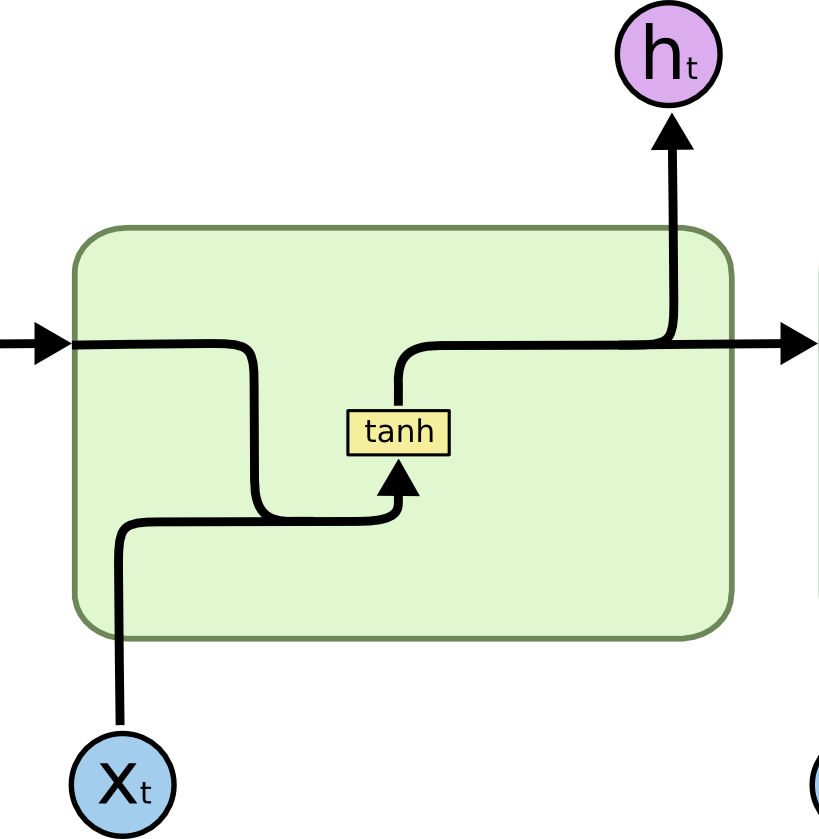
\includegraphics[scale=0.5]{rnn/rnn_cell}
	\end{center}
	\caption{A single RNN cell. From~\cite{olah2015understanding}\label{fig:rnn_cell}}
\end{figure}

As can be seen in figure~\ref{fig:rnn_cell}, RNNs only have a single vector that functions as the hidden state and the cell's output. The vector of values at the output of the hidden layer that are observed at time \(t\), h\(_{\text{t}}\) is calculated by the following function where h\(_{\text{t}}\) is the current hidden state vector and h\(_{\text{t-1}}\) the vector of the previous hidden state, \(W\) is the weight matrix for the cell's input, \(U\) is the weight matrix for the hidden value, x\(_{\text{t}}\) is the input of this cell, and \(\sigma \) is a sigmoid function used to squash its inputs into the [0, 1] range:

\begin{equation} \label{eq:something}
h_t = \sigma(Wx_t + Uh_\text{t-1})
\end{equation}

%cSpell:words pascanu
These standard RNN cells and any other RNN architectures could be stacked on top of each other. These are also known as deep recurrent neural networks. In~\cite{pascanu2013construct}, deep RNNs were shown to outperform conventional single-layer RNNs at polyphonic music prediction and language modeling. An RNN architecture that takes advantage of the stacking of layers in particular is the Depth Gated RNN, introduced in~\cite{yao2015depth}, which uses an additional depth gate to connect memory cells of adjacent layers.

\section{LSTMs}

The LSTM architecture, contrary to regular RNNs, has an additional hidden state that is never directly outputted (see figure~\ref{fig:lstm_cell}). This additional hidden state can then be used by the network solely for remembering previous relevant information. Instead of having to share its \enquote{memory} with its output, these values are now separate. During the training process, an LSTM learns what should be remembered for the future and what should be forgotten, which is achieved by using its internal weights.

\begin{figure}[H]
	\begin{center}
		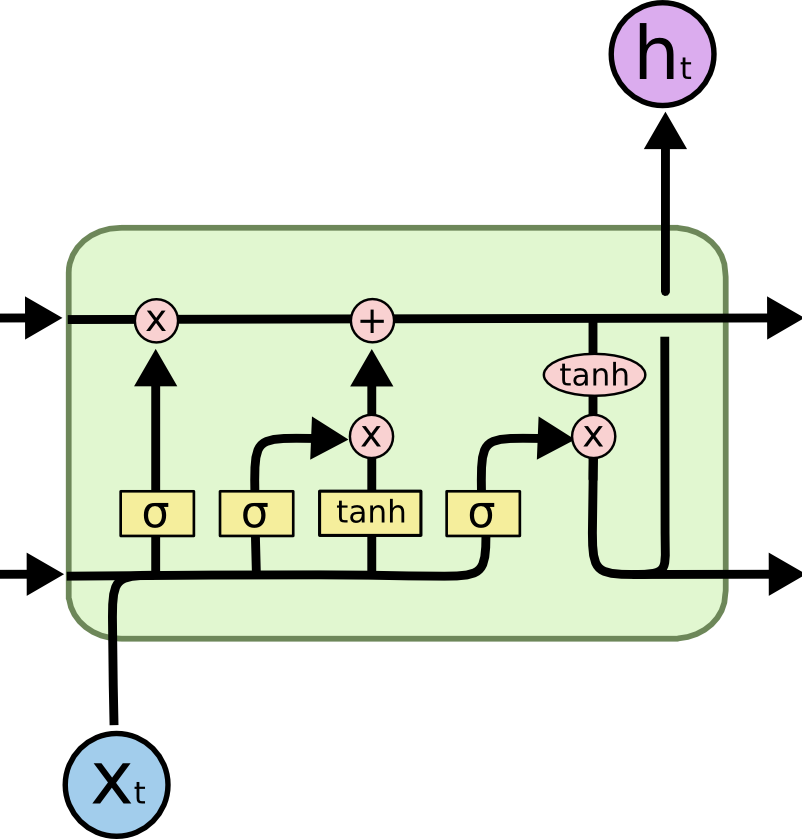
\includegraphics[scale=0.5]{rnn/lstm_cell}
	\end{center}
	\caption{A single LSTM cell. From~\cite{olah2015understanding}\label{fig:lstm_cell}}
\end{figure}

As can be seen in the figure, there are quite a few more parameters in this cell than in a normal RNN cell. The calculation of the output vector and the hidden vector involves several operations, a full explanation of which can be found in~\cite{olah2015understanding}. First of all the network determines how much of the hidden state to forget, also called the forget gate. This is done by pushing both the previous iteration's output (\(c_{t-1}\)) and the forget gate vector (\(f_t\)) through a matrix multiplication. This allows the network to forget values at specific indices in the previous iteration's output vector. \(f_t\) can be obtained by using formula~\ref{eq:forget_vector_lstm}, where \(W\) contains the weights for the input and \(U\) contains the weights for the previous iteration's output vector, \(x_t\) refers to the input, \(h_{t-1}\) to the previous iteration's output vector and \(b\) to a set of bias vectors:

\begin{equation} \label{eq:forget_vector_lstm}
f_t = \sigma(W_f x_t + U_f h_{t-1} + b_f)
\end{equation}

The network then determines what to remember from the input vector. This is commonly referred to as the input gate. This is done by pushing the previous forget gate's output as well as the input gate through a matrix addition function. The output of the input gate (\(i_t\)) can be found by using the following formula:

\begin{equation} \label{eq:input_vector_lstm}
i_t = \sigma(W_i x_t + U_i h_{t-1} + b_i)
\end{equation}

The final hidden state vector (\(c_t\)) can then be found by using the previous two results as follows, where \(\circ \) denotes the Hadamard product (where each value at index \(ij\) is the product of the values at the indices \(ij\) in the two input matrices): 

\begin{equation} \label{eq:hidden_state_vector_lstm}
c_t = f_t \circ c_{t-1} + i_t \circ \sigma(W_c x_t + U_c h_{t-1} + b_c)
\end{equation}

This vector is then passed on to the next iteration. Now the output gate vector \(o_t\) is calculated:

\begin{equation} \label{eq:something}
o_t = \sigma(W_o x_t + U_o h_{t-1} + b_o)
\end{equation}

The output state \(h_t\) can then be obtained:

\begin{equation} \label{eq:something}
h_t = o_t \circ \sigma(c_t)
\end{equation}

%cSpell:words gers jozefowicz kingma
This results in a version of an RNN that is able to remember more and is more liberal in choosing what information it wants to keep in the hidden state and what it wants to discard. This makes LSTM networks better suited for tasks involving series of data. This has lead to the LSTM architecture becoming the dominant RNN architecture. 

\section{GRUs}
Another RNN architecture is the Gated Recurrent Unit (GRU), introduced in~\cite{cho2014learning}. This architecture combines the input and forget gates into a single so-called \enquote{update gate} and also merges the cell state and hidden state (see figure~\ref{fig:gru_cell}). The calculation of the merged output vector once again consists of several operations. The network first computes the \enquote{reset gate} \(r_t\) using the following function, where \(W_r\) are the weights for the reset gate and \([h_{t-1}, x_t]\) signifies the concatenation of \(h_{t-1}\) and \(x_t\):

%cSpell:words olah
\begin{figure}
	\begin{center}
		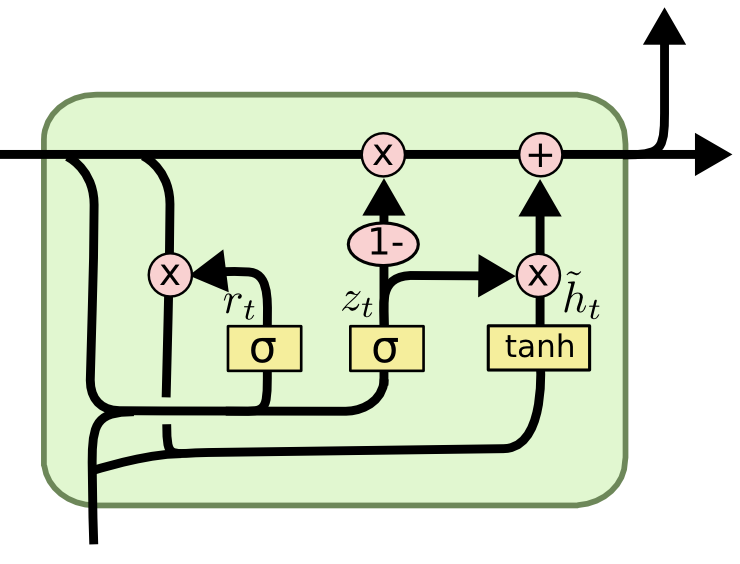
\includegraphics[scale=0.5]{rnn/gru_cell}
	\end{center}
	\caption{A single GRU variation cell. From~\cite{olah2015understanding}\label{fig:gru_cell}}
\end{figure}

\begin{equation} \label{eq:gru_reset_gate}
r_t = \sigma(W_r [h_{t-1}, x_t])
\end{equation}

After this, the \enquote{update gate} \(z_t\) is computed as follows, where \(W_z\) holds the weights of the update gate:

\begin{equation} \label{eq:gru_update_gate}
z_t = \sigma(W_z [h_{t-1}, x_t])
\end{equation}

The output vector \(h_t\) (representing both the cell's output and its state) can then be computed by the following function:

\begin{equation} \label{eq:gru_output}
h_t = (1 - z_t) * h_{t-1} + z_t * \tilde{h_t}
\end{equation}

Where \(\tilde{h_t}\) is computed by:

\begin{equation} \label{eq:gru_output_partial}
\tilde{h_t} = \tanh(W * [r_t * h_{t-1}, x_t])
\end{equation}

\section{Architectures}

There have been numerous variations of the standard LSTM architecture that was just described, including but not limited to the Peephole LSTM~\cite{gers2002learning} that connects the hidden state with the gate activation functions, and the Neural Turing Machine~\cite{graves2014neural}, which extends the capabilities of the neural network by coupling it to an external memory resource.

There has been some research into which architectures are the most efficient. Some architectures are better than others at specific problems, as~\cite{jozefowicz2015empirical} demonstrates. However, this study did not include a variation of anomaly detection in its testing problems. This means that experiments regarding what architecture is the most promising for anomaly detection still have to be done. Experiments regarding the architecture of the system are done in Chapter~\ref{ch:experiments}. The base architecture that will be used in this thesis will be the standard LSTM architecture. Since it is the dominant architecture and has seen a lot of use, testing other architectures against this baseline seems like a good choice. For training the \enquote{adam} optimizer will be used, which was introduced in~\cite{kingma2014adam}. This is a method of gradient-based optimization of stochastic objective functions.